
\section{Introduction}
Summary of the Python code used for processing and analyzing structural connectivity (SC) and functional connectivity (FC) matrices. Various tasks were performed including loading data, preprocessing, visualization, and community detection.

\section{Data Extraction}

\begin{enumerate}
    \item \textbf{Loading Data:} 
    The data was loaded from .mat files using the \texttt{scipy.io.loadmat} function. This function reads the MATLAB files and loads the data into Python variables.
    
    \item \textbf{Extracting SC and FC Data:} 
    After loading the .mat files, the SC (Structural Connectivity) and FC (Functional Connectivity) data were extracted from the loaded data structures. This was done by accessing specific keys within the loaded data that correspond to SC and FC.
    
    \item \textbf{Extracting Age Group Matrices:} 
    The SC and FC data contain matrices for different age groups (young, adult, old). These matrices were extracted by accessing the specific fields within the SC and FC data structures and each age group's data was stored separately.
\end{enumerate}


\section{Preprocessing}
Preprocessed matrices to set negative weights to zero, apply thresholding, and normalize.

Visualized matrices as heatmaps and histograms using \texttt{matplotlib}. For example, iterated over the matrices for different age groups and displayed them using the \texttt{imshow} function with the 'viridis' colormap. Added colorbars to each subplot for better interpretation.

\begin{figure}[h!]
    \centering
    \begin{subfigure}[b]{0.45\textwidth}
        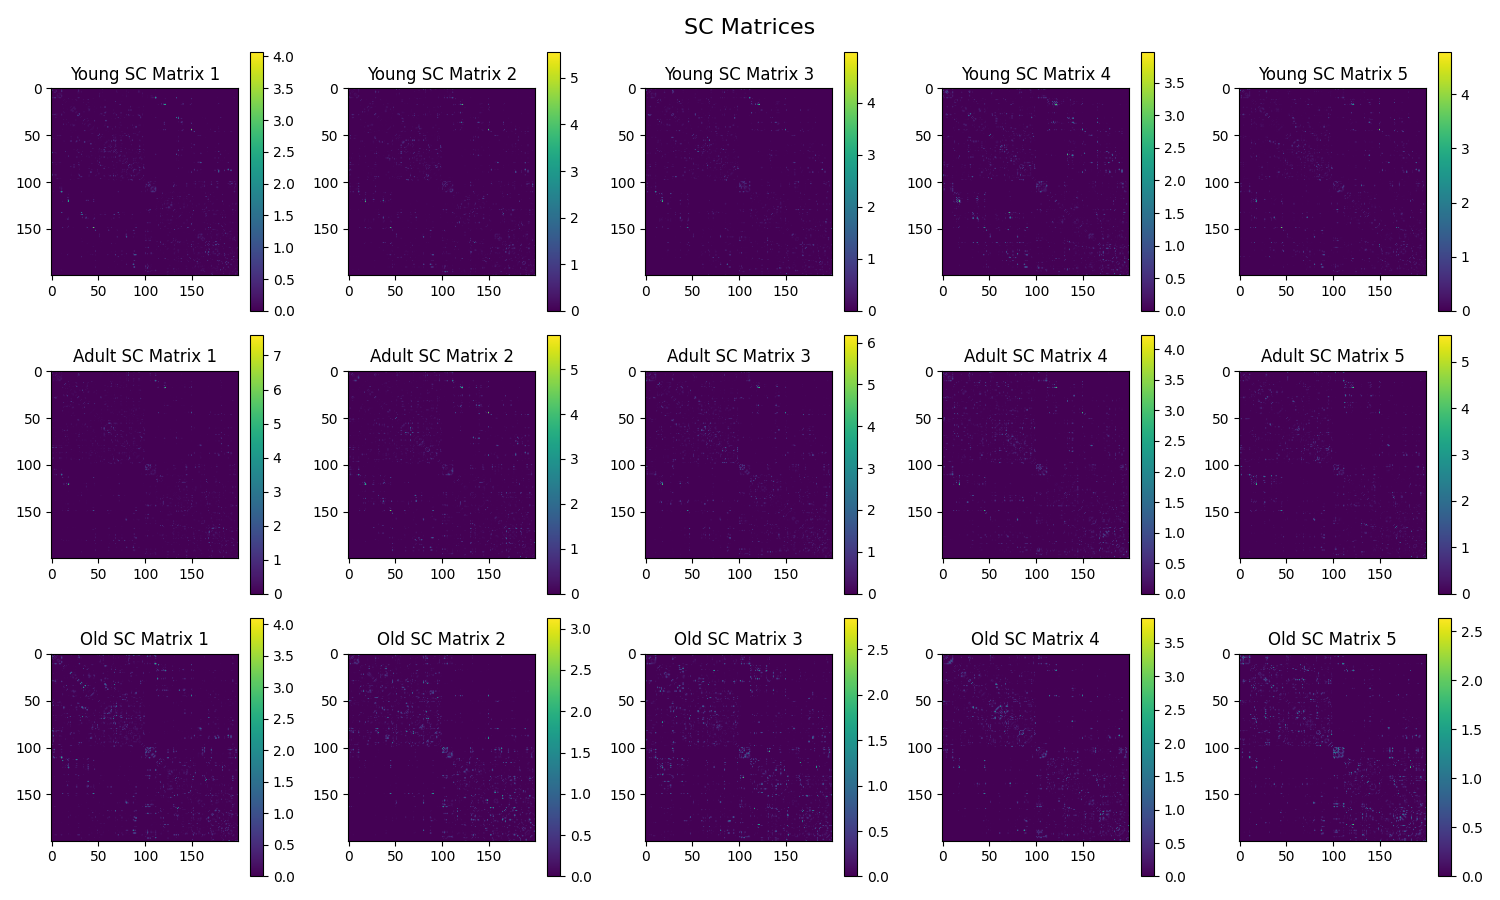
\includegraphics[width=\textwidth]{C:/Users/barbo/Desktop/thesis repo clone/thesis/Thesis Draft/figures/SC_matrices_heatmap.png}
        \caption{Heatmap of Original SC Matrices}
    \end{subfigure}
    \begin{subfigure}[b]{0.45\textwidth}
        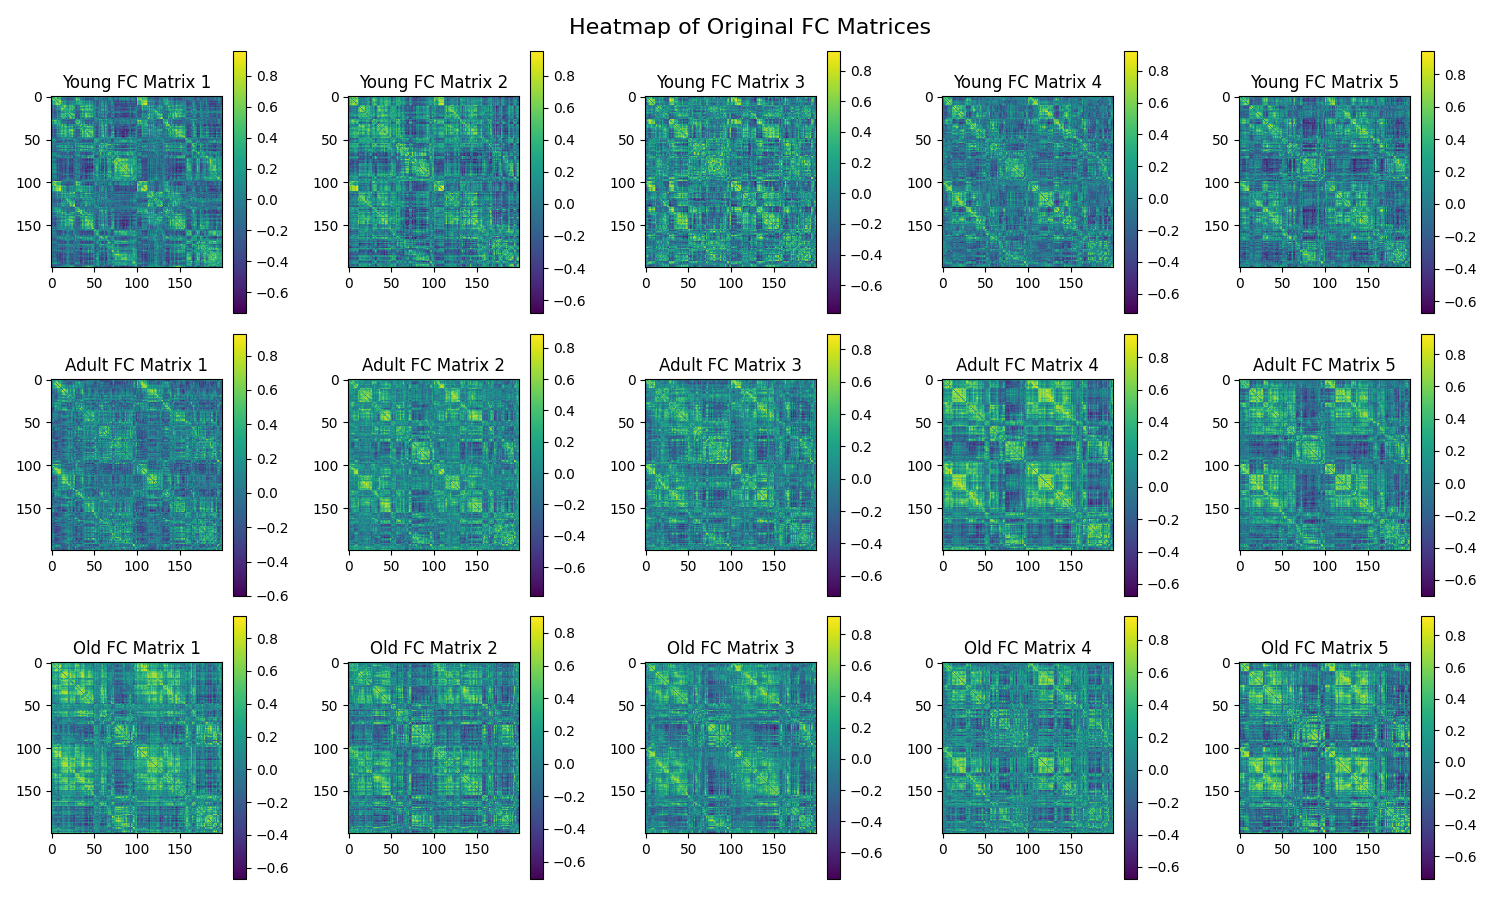
\includegraphics[width=\textwidth]{C:/Users/barbo/Desktop/thesis repo clone/thesis/Thesis Draft/figures/FC_matrices_heatmap.png}
        \caption{Heatmap of Original FC Matrices}
    \end{subfigure}
    \begin{subfigure}[b]{0.45\textwidth}
        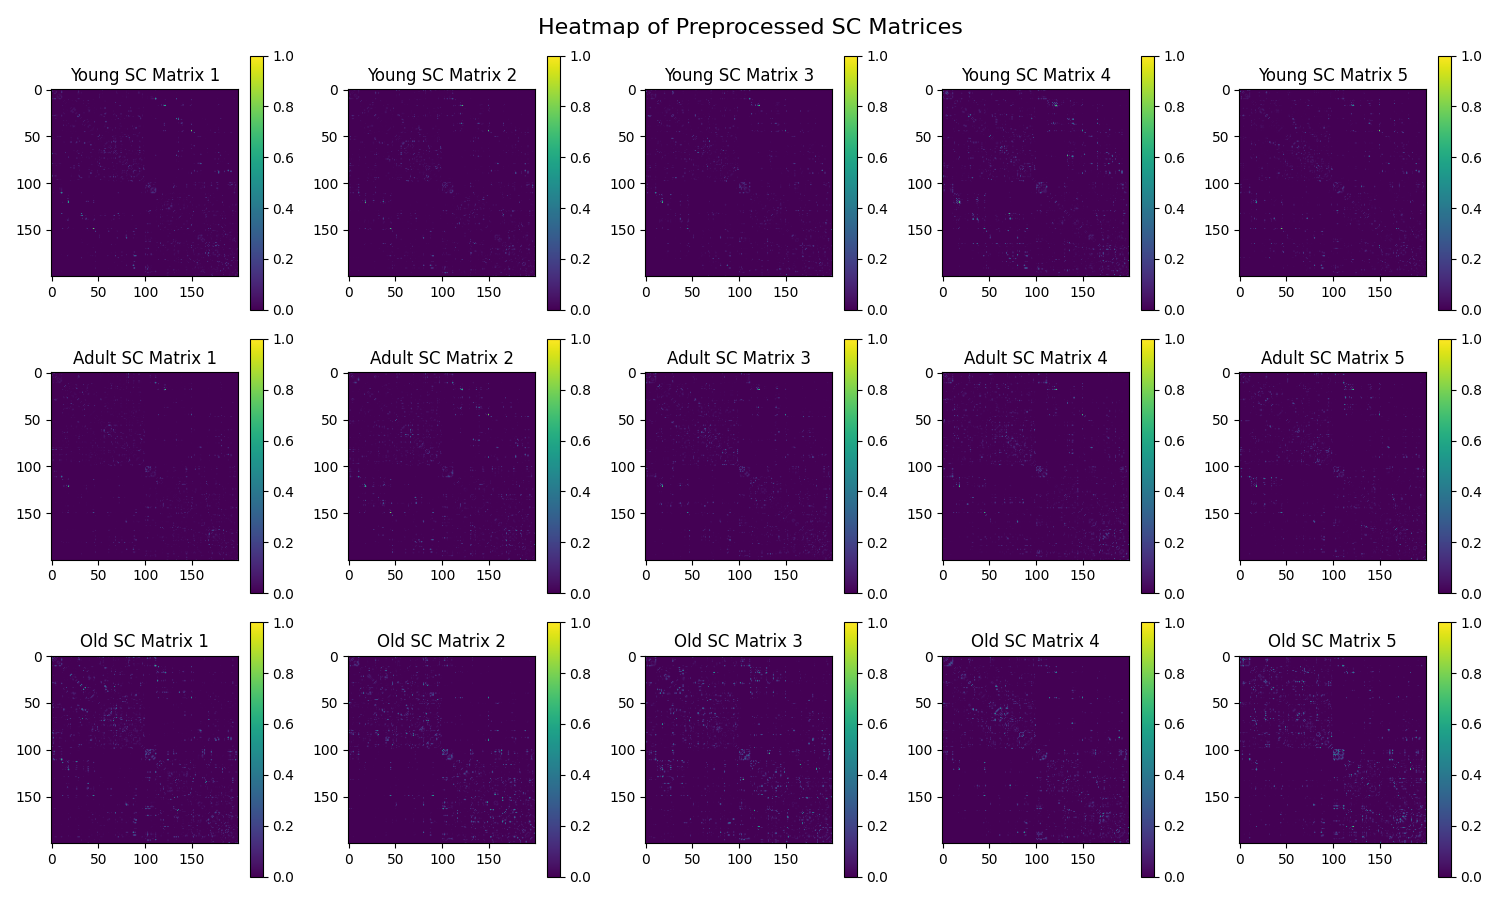
\includegraphics[width=\textwidth]{C:/Users/barbo/Desktop/thesis repo clone/thesis/Thesis Draft/figures/SC_matrices_heatmap_preprocessed.png}
        \caption{Heatmap of Preprocessed SC Matrices}
    \end{subfigure}
    \begin{subfigure}[b]{0.45\textwidth}
        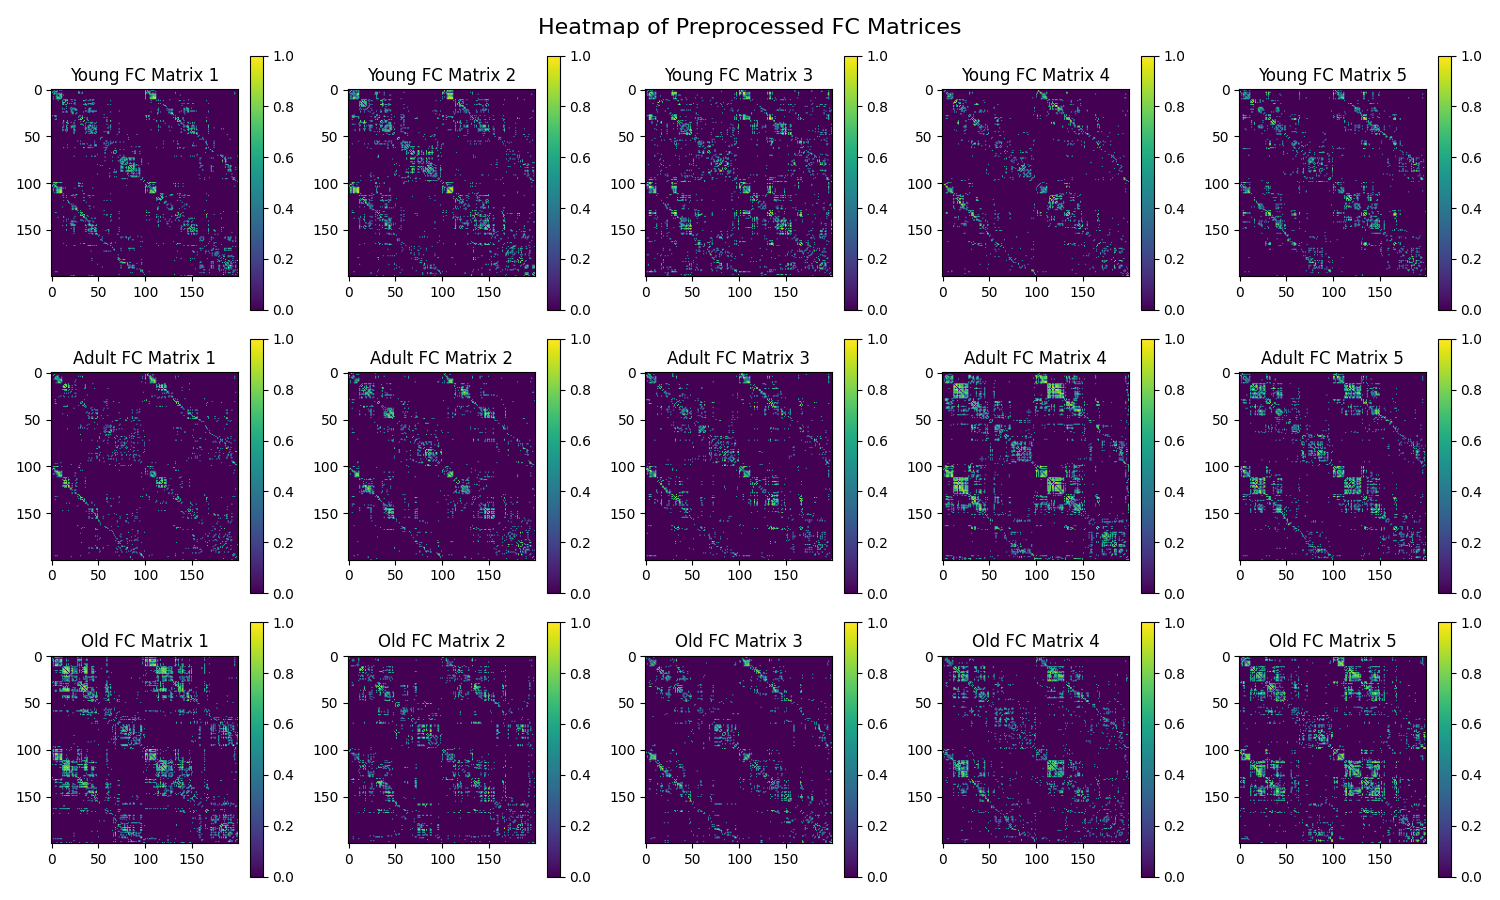
\includegraphics[width=\textwidth]{C:/Users/barbo/Desktop/thesis repo clone/thesis/Thesis Draft/figures/FC_matrices_heatmap_preprocessed.png}
        \caption{Heatmap of Preprocessed FC Matrices}
    \end{subfigure}
    \caption{Various Heatmaps of SC and FC Matrices}
\end{figure}


\begin{figure}[h!]
    \centering
    \begin{subfigure}[b]{0.45\textwidth}
        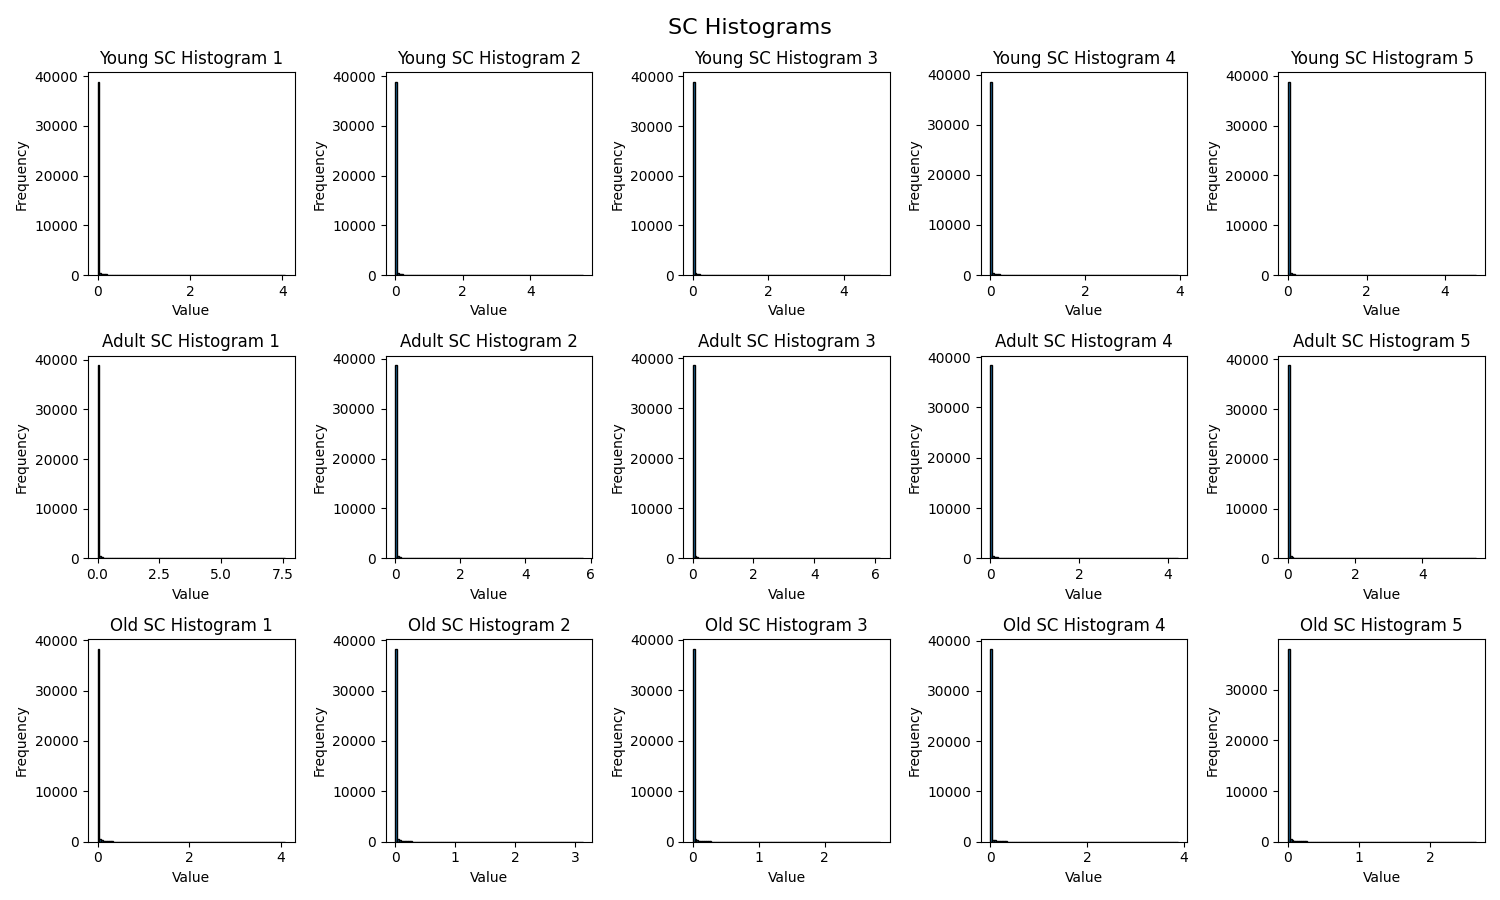
\includegraphics[width=\textwidth]{C:/Users/barbo/Desktop/thesis repo clone/thesis/Thesis Draft/figures/SC_matrices_histogram.png}
        \caption{Histogram of Original SC Matrices}
    \end{subfigure}
    \begin{subfigure}[b]{0.45\textwidth}
        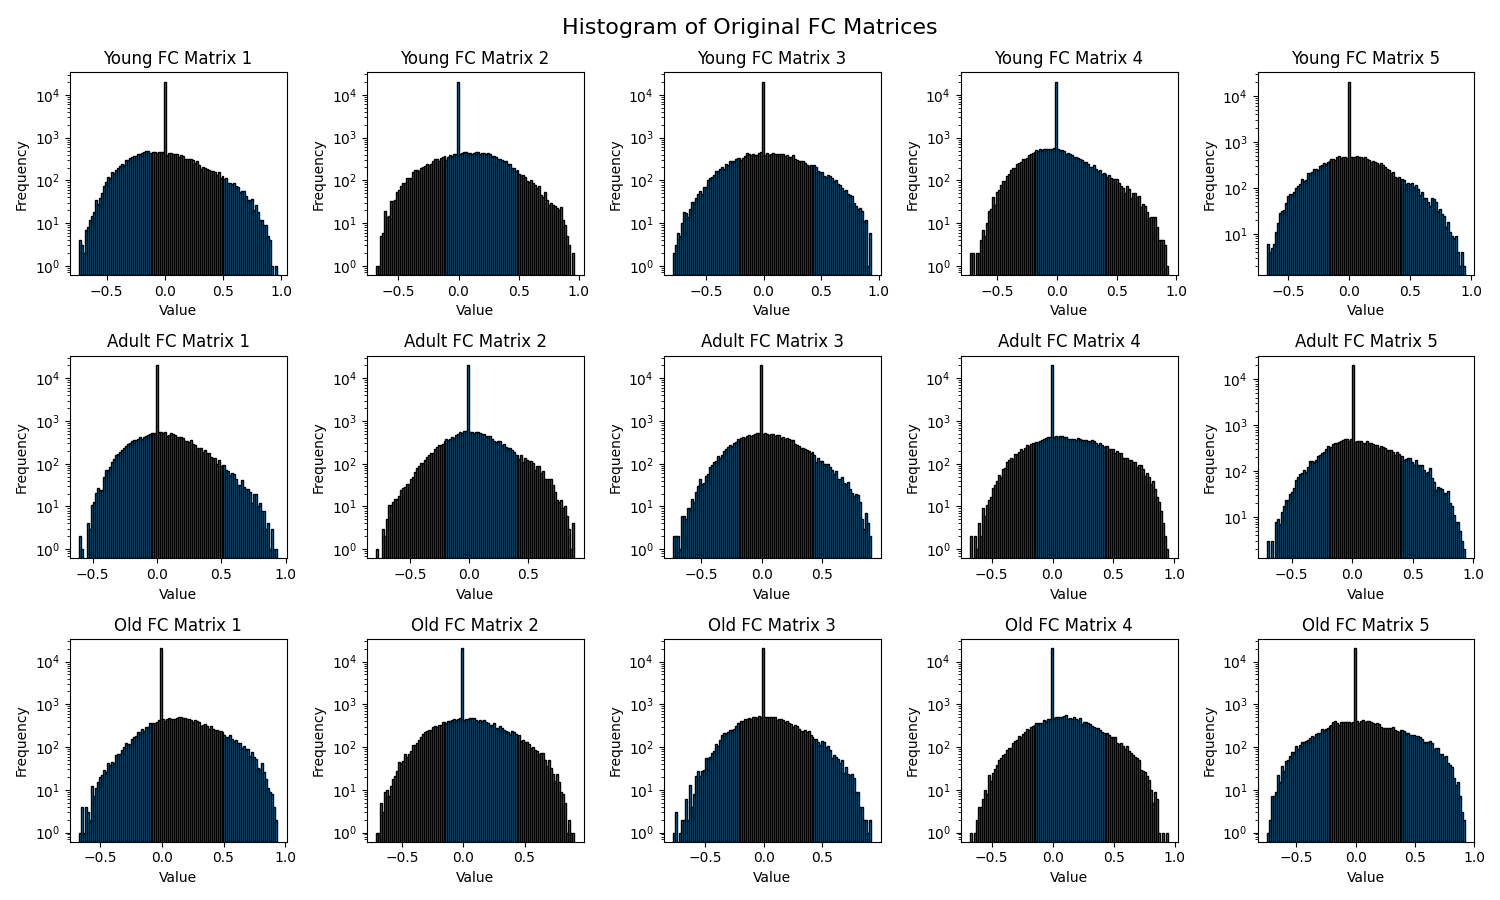
\includegraphics[width=\textwidth]{C:/Users/barbo/Desktop/thesis repo clone/thesis/Thesis Draft/figures/FC_matrices_histogram.png}
        \caption{Histogram of Original FC Matrices}
    \end{subfigure}
    \begin{subfigure}[b]{0.45\textwidth}
        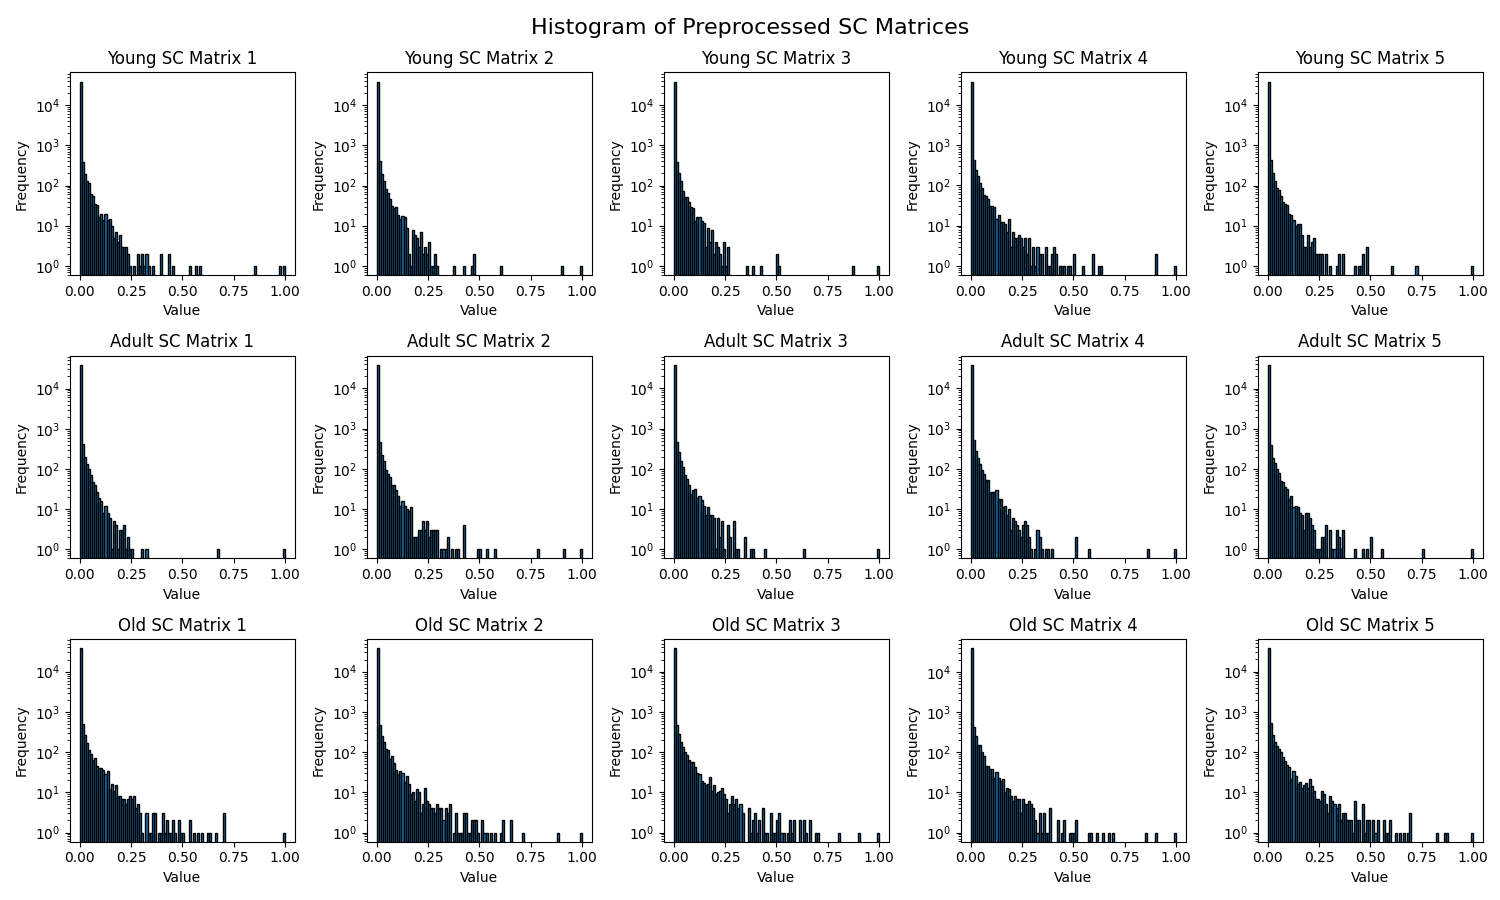
\includegraphics[width=\textwidth]{C:/Users/barbo/Desktop/thesis repo clone/thesis/Thesis Draft/figures/SC_matrices_histogram_preprocessed.png}
        \caption{Histogram of Preprocessed SC Matrices}
    \end{subfigure}
    \begin{subfigure}[b]{0.45\textwidth}
        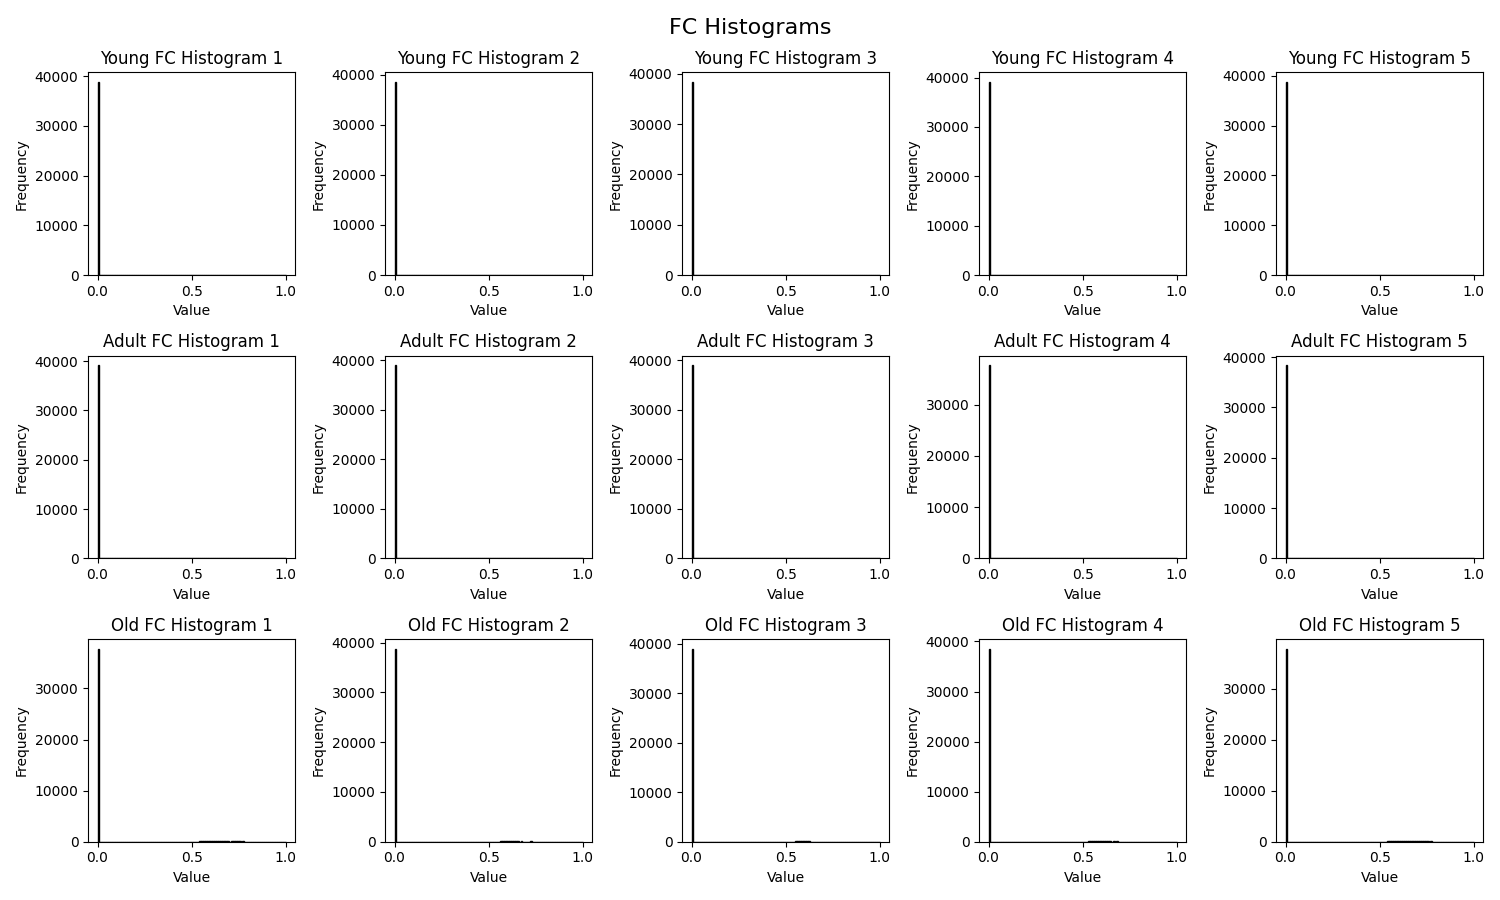
\includegraphics[width=\textwidth]{C:/Users/barbo/Desktop/thesis repo clone/thesis/Thesis Draft/figures/FC_matrices_histogram_preprocessed.png}
        \caption{Histogram of Preprocessed FC Matrices}
    \end{subfigure}
    
    \caption{Various Histograms of SC and FC Matrices}
\end{figure}


\section{Conversion and Preprocessing of Graphs}
Converted matrices to graphs using \texttt{networkx}. Preprocessed graphs by removing self-loops, isolates, and small disconnected components.

\section{Community Detection}
Applied the Louvain method for community detection on the preprocessed graphs using the \texttt{community} package.

\section{Visualization of Graphs}
Visualized and saved graphs, including those with detected communities. Used the spring layout algorithm for graph visualization to position the nodes. 

\begin{figure}[h!]
    \centering
    \begin{subfigure}[b]{0.45\textwidth}
        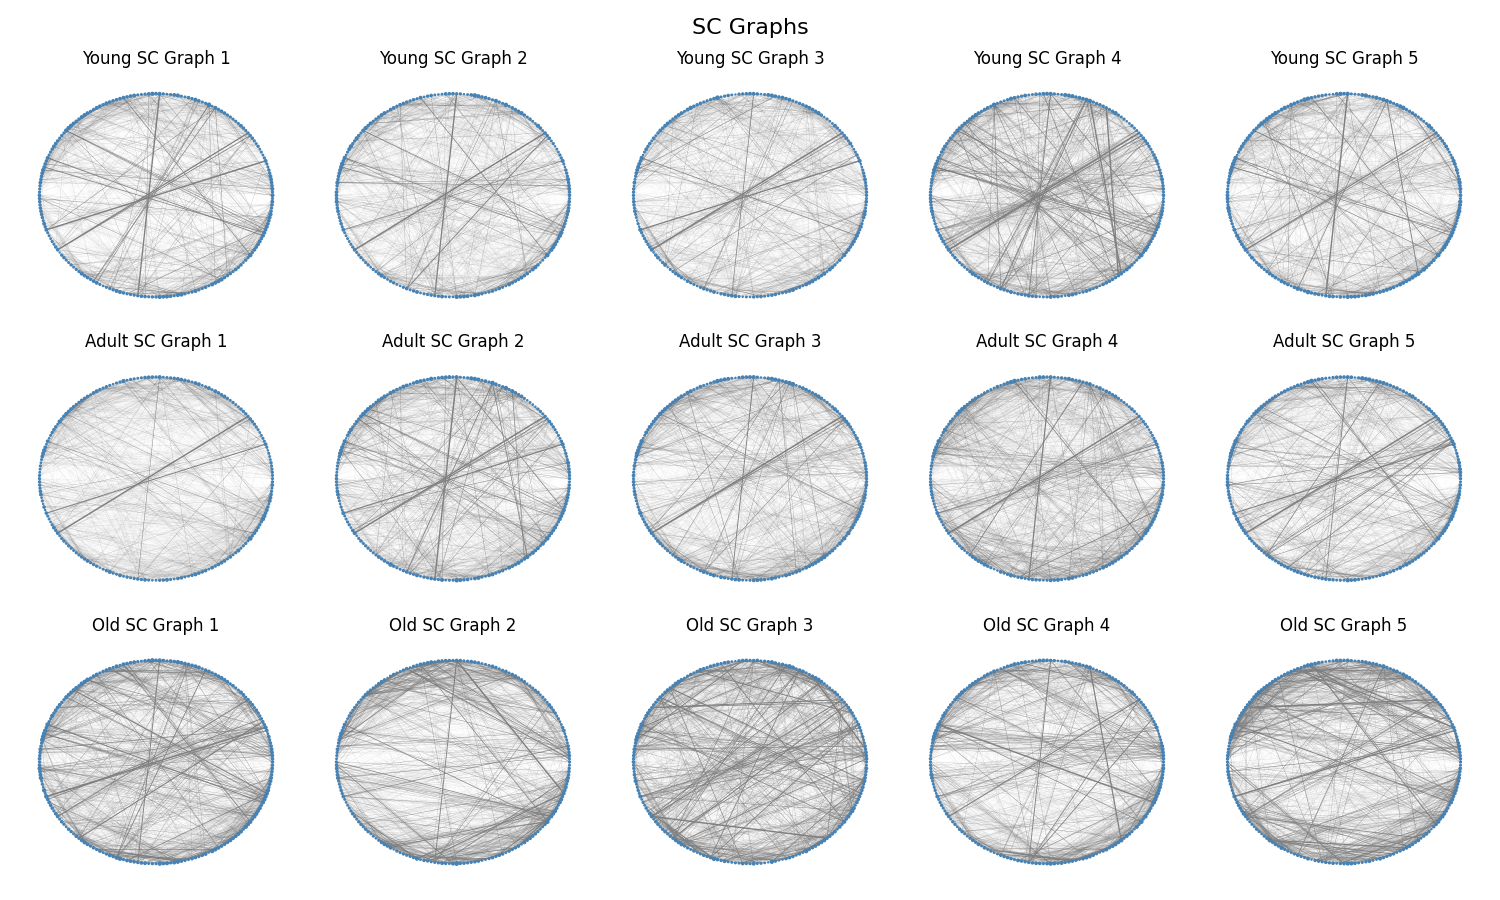
\includegraphics[width=\textwidth]{C:/Users/barbo/Desktop/thesis repo clone/thesis/Thesis Draft/figures/SC_graphs.png}
        \caption{Original SC Graphs}
    \end{subfigure}
    \begin{subfigure}[b]{0.45\textwidth}
        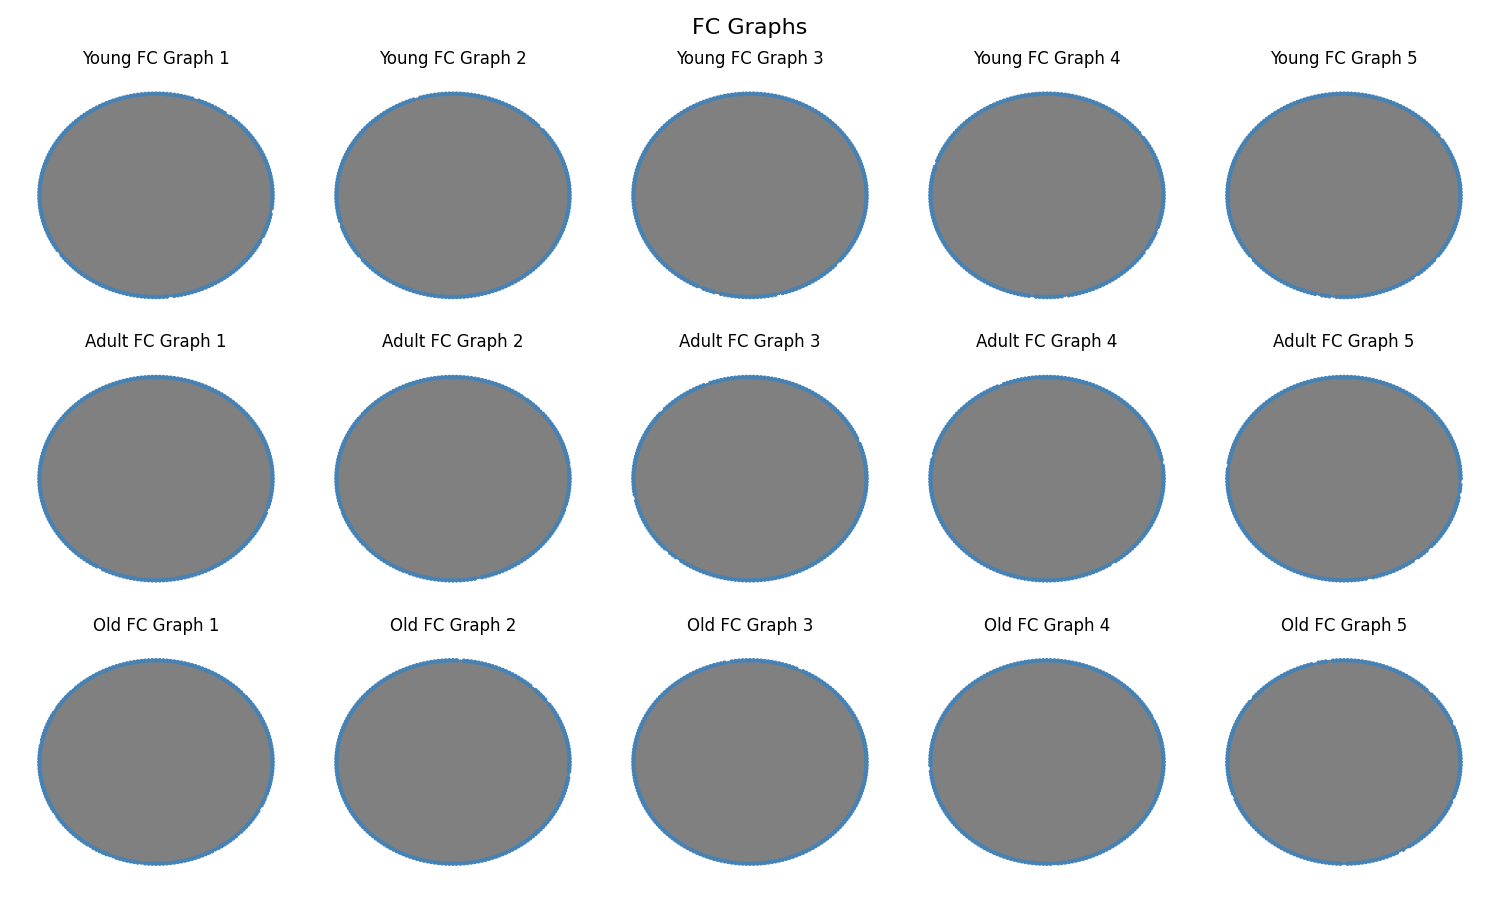
\includegraphics[width=\textwidth]{C:/Users/barbo/Desktop/thesis repo clone/thesis/Thesis Draft/figures/FC_graphs.png}
        \caption{Original FC Graphs}
    \end{subfigure}
    
    \begin{subfigure}[b]{0.45\textwidth}
        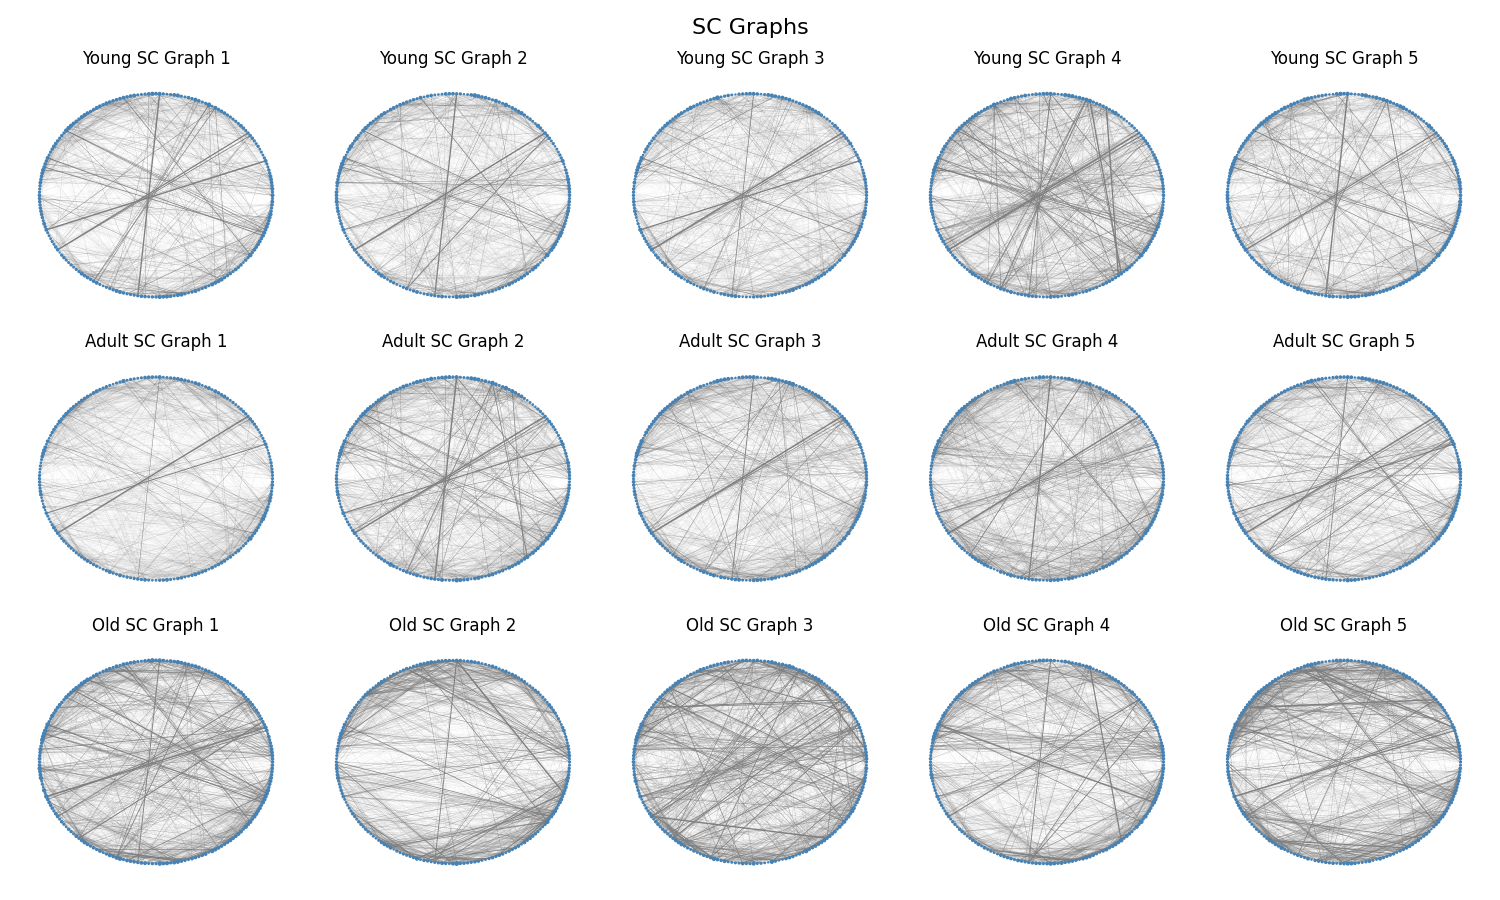
\includegraphics[width=\textwidth]{C:/Users/barbo/Desktop/thesis repo clone/thesis/Thesis Draft/figures/SC_graphs_preprocessed.png}
        \caption{Preprocessed SC Graphs}
    \end{subfigure}
    \begin{subfigure}[b]{0.45\textwidth}
        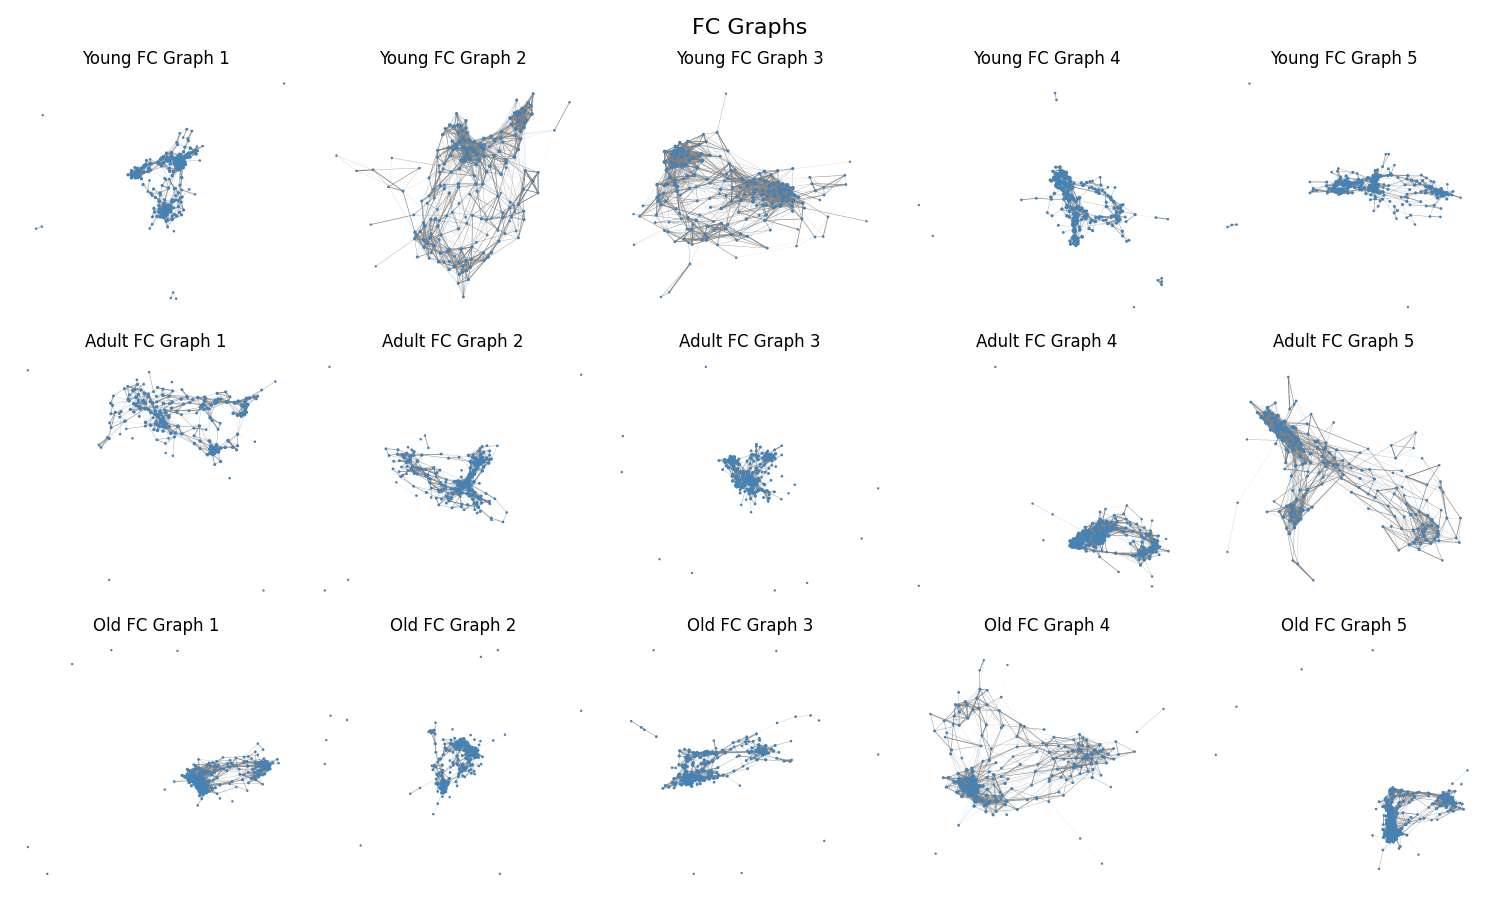
\includegraphics[width=\textwidth]{C:/Users/barbo/Desktop/thesis repo clone/thesis/Thesis Draft/figures/FC_graphs_preprocessed.png}
        \caption{Preprocessed FC Graphs}
    \end{subfigure}
    
    \begin{subfigure}[b]{0.45\textwidth}
        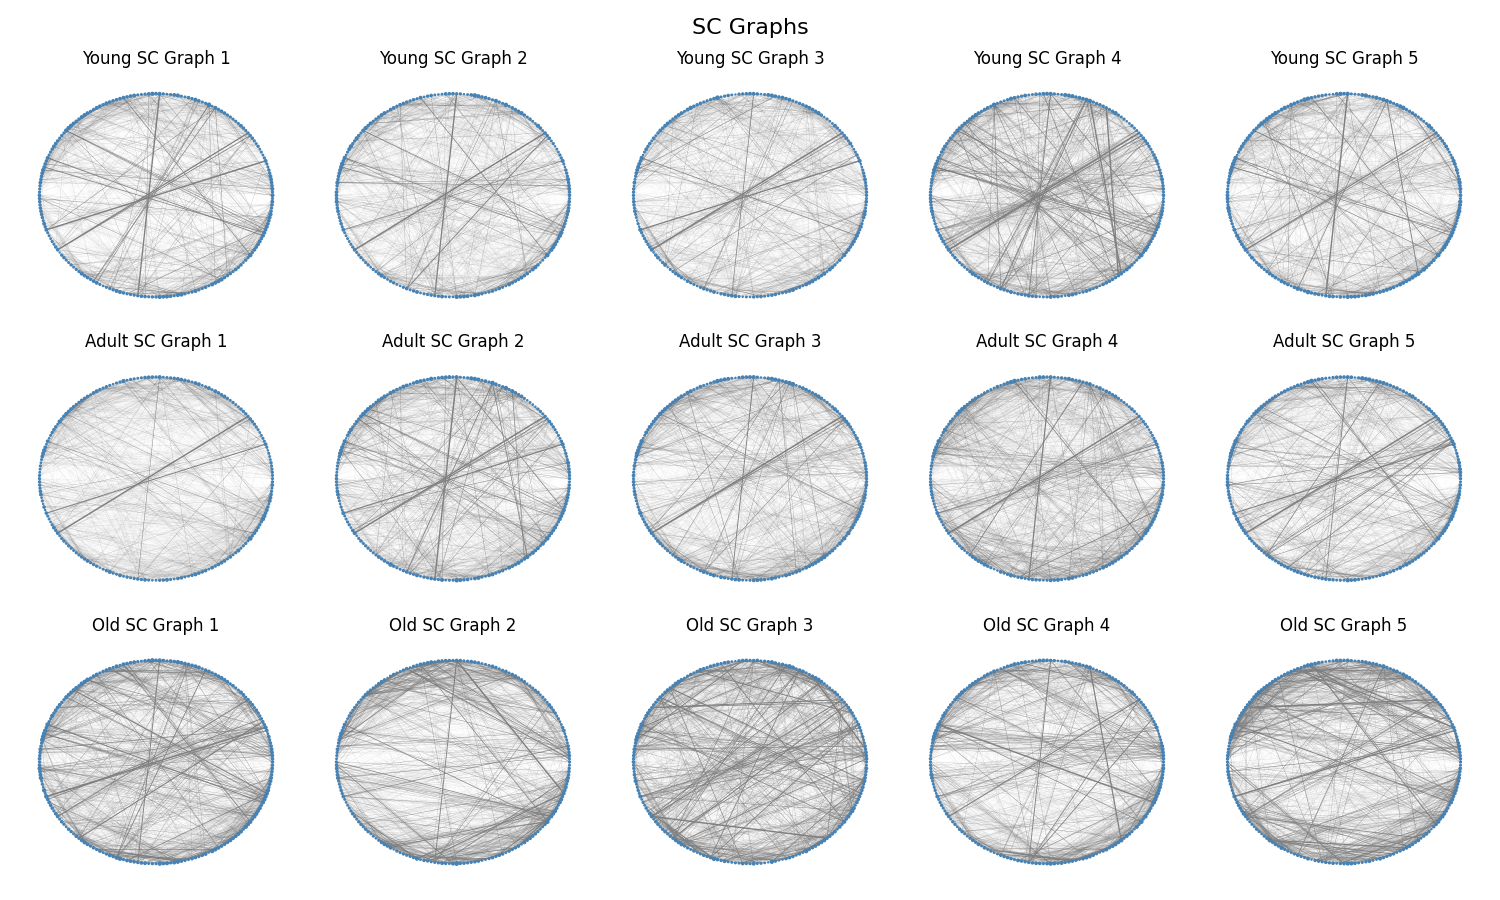
\includegraphics[width=\textwidth]{C:/Users/barbo/Desktop/thesis repo clone/thesis/Thesis Draft/figures/SC_graphs_preprocessed_louvain.png}
        \caption{Louvain Preprocessed SC Graphs}
    \end{subfigure}
    \begin{subfigure}[b]{0.45\textwidth}
        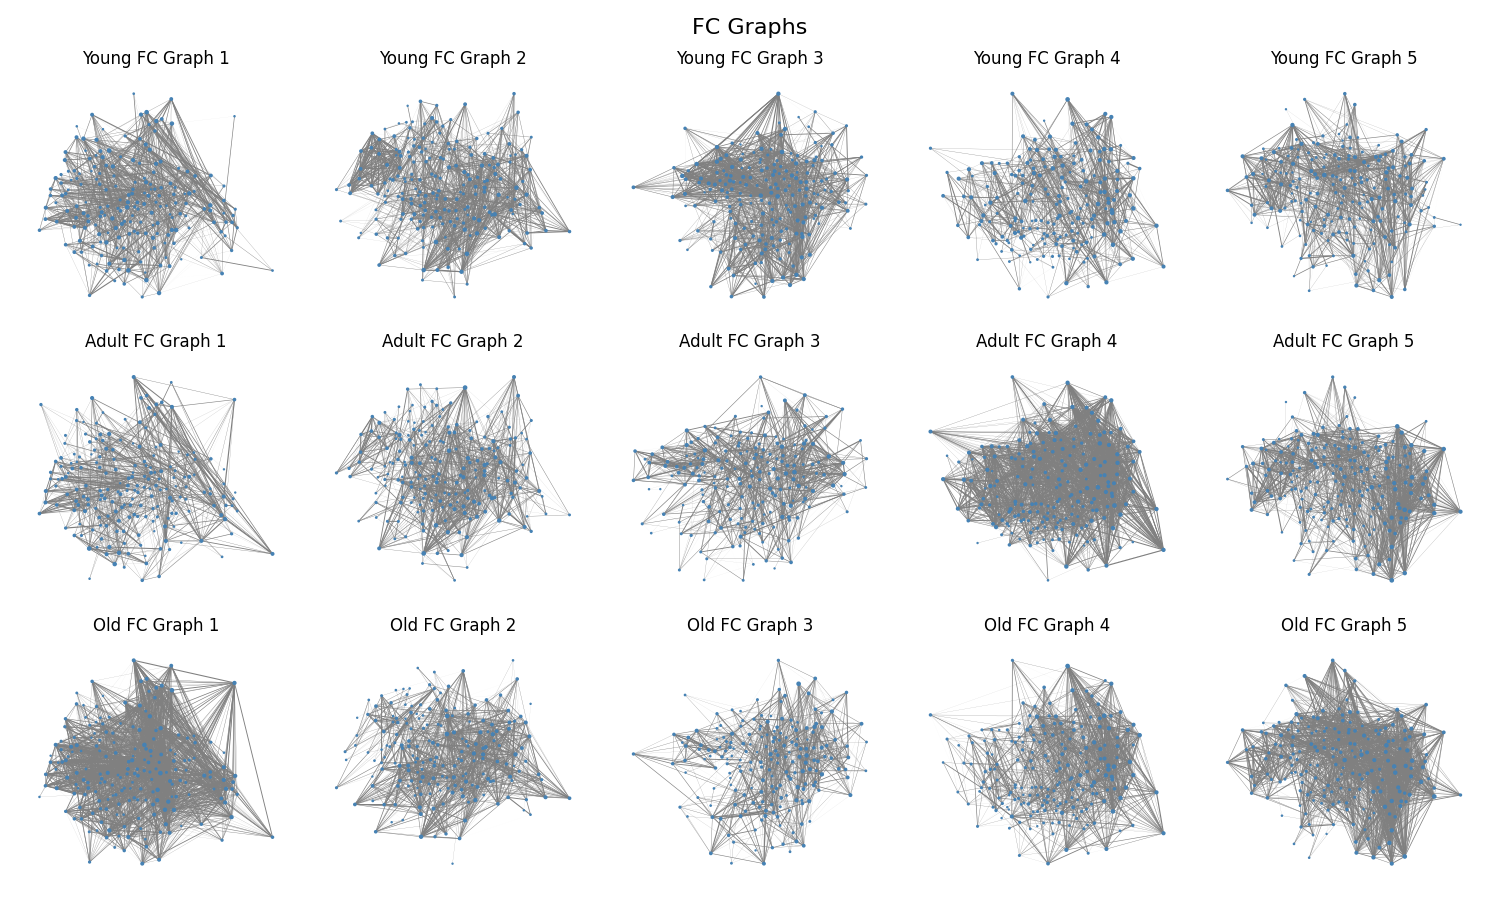
\includegraphics[width=\textwidth]{C:/Users/barbo/Desktop/thesis repo clone/thesis/Thesis Draft/figures/FC_graphs_preprocessed_louvain.png}
        \caption{Louvain Preprocessed FC Graphs}
    \end{subfigure}
    
    \begin{subfigure}[b]{0.45\textwidth}
        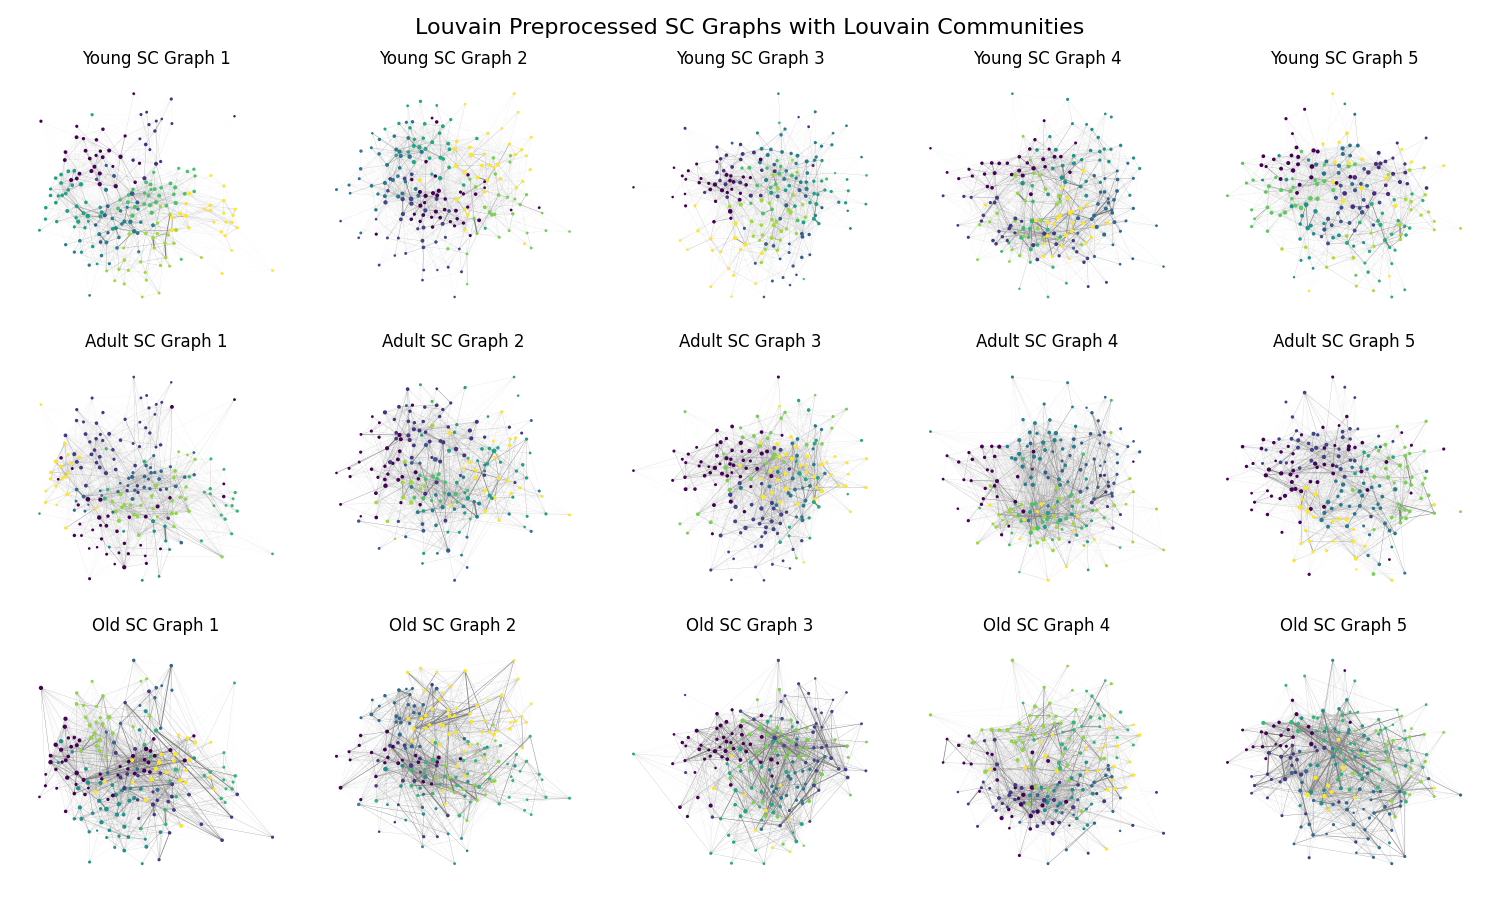
\includegraphics[width=\textwidth]{C:/Users/barbo/Desktop/thesis repo clone/thesis/Thesis Draft/figures/SC_graphs_preprocessed_louvain_communities.png}
        \caption{Louvain Preprocessed SC Graphs with Louvain Communities}
    \end{subfigure}
    \begin{subfigure}[b]{0.45\textwidth}
        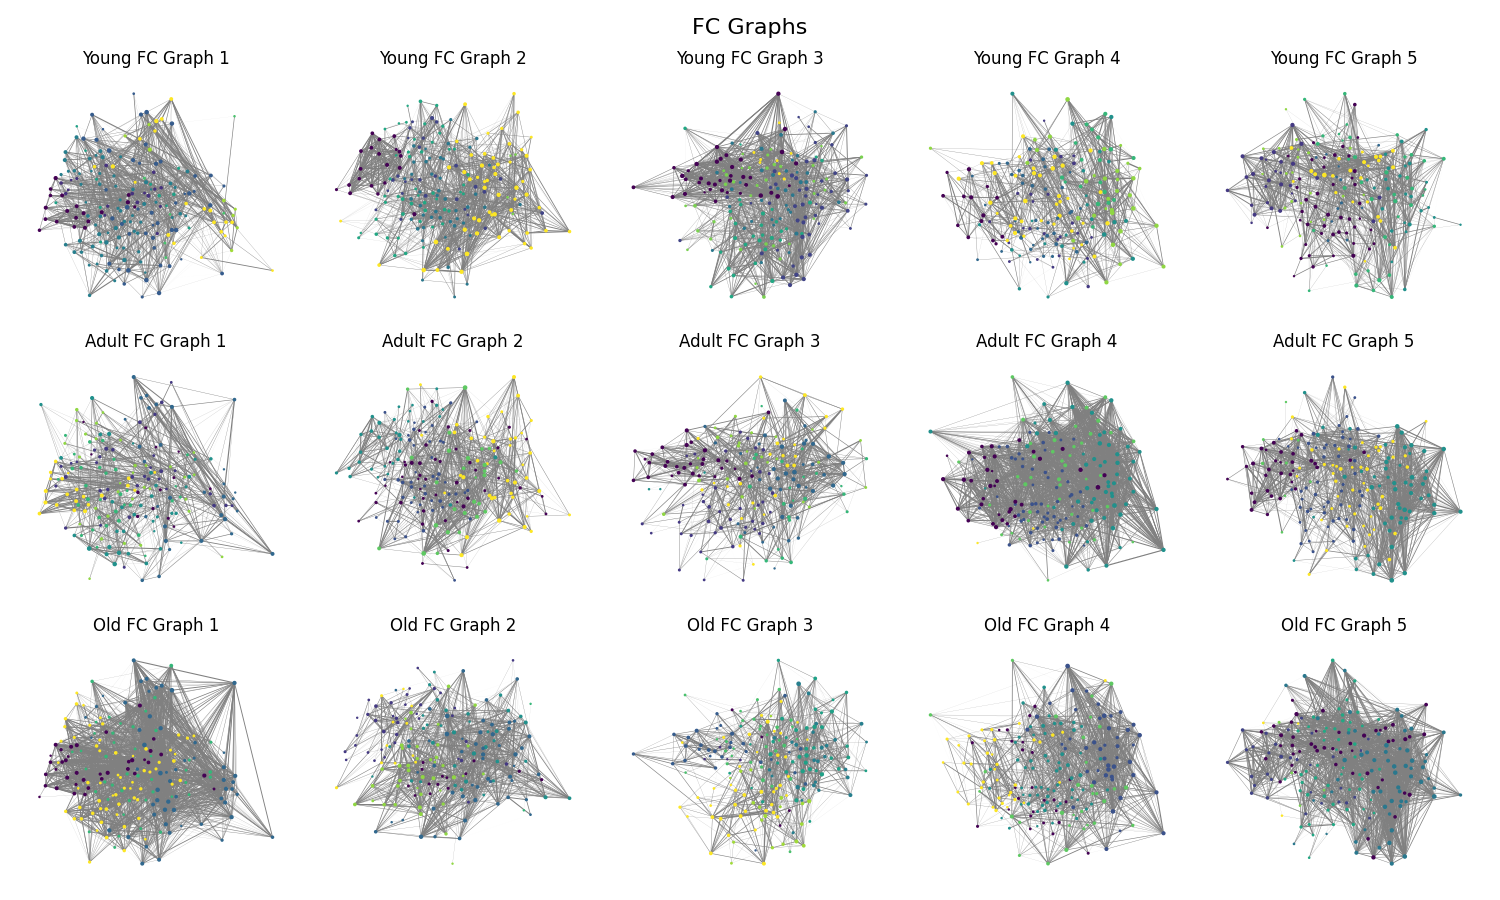
\includegraphics[width=\textwidth]{C:/Users/barbo/Desktop/thesis repo clone/thesis/Thesis Draft/figures/FC_graphs_preprocessed_louvain_communities.png}
        \caption{Louvain Preprocessed FC Graphs with Louvain Communities}
    \end{subfigure}
    
    \caption{Various Graphs of SC and FC Matrices}
\end{figure}


\section{Conclusion}
Created a pipeline for loading, preprocessing, visualizing, and analyzing SC and FC matrices. Used various visualization techniques and community detection methods for in-depth analysis of the connectivity patterns.








